\section{Wikitty Publication Site}

La partie site de Wikitty Publication concerne des fonctionnalités
destinées à l'administration et les éléments coeur du moteur de publication
comme l'interprétation du code contenu dans les WikittyPubText. 

Ces fonctionnalités principales sont :
\begin{itemize}
\item Raw, qui permet l'affichage des WikittyPubData exemple des images
\item Edit, qui permet de créer ou d'éditer des Wikitty
\item Eval, qui permet l'évaluation du code contenu dans un WikittyPubText
\item View, qui permet l'affichage et la recherche des Wikitty
\end{itemize}

Un premier prototype avait été réalisé c'était la base de travail, ce prototype
était fait avec des jsp/servlet simplement sans support d'un quelconque
framework comme struts.

Le travail sur cette partie de publication se concentrait donc sur
l'amélioration de ce prototype sous différent aspect.


\subsection{Migration vers struts}

Le premier aspect de l'amélioration du prototype était de migrer les jsp/servlet
vers le framework struts. Struts est un donc un framework qui permet un bon
support du modèle MVC pour les applications web.

Struts permet au dévelloppeurs de se concentrer sur la vue et le modèle de son
application Web, à la charge de struts l'aspect contrôleur du modèle MVC. En
effet on peut définir l'enchainement des actions effectuées et la page qui sera
affiché en conséquence.

Dans struts on parle d'action, de package et d'intercepteur, les packages
regroupent les actions et les piles d'intercepteurs, ces packages peuvent en
étendre d'autre et donc hériter de leurs propriétés. Les packages peuvent
posséder un 'namespace' qui leur permet d'être défini pour un sous espace de
l'application.

\begin{figure}[!ht]
\centering
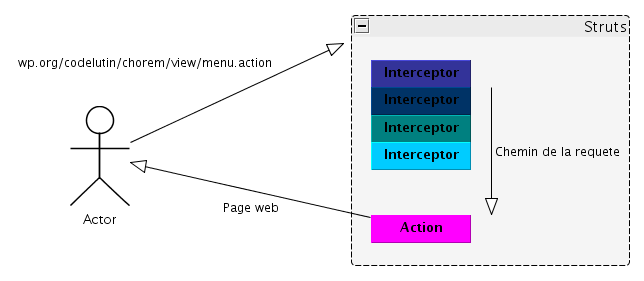
\includegraphics[height=6cm,width=17cm]{image/strutsexplain.png}
  		\caption{Diagramme Struts}
  		\label{diagstruts}
\end{figure}

Les intercepteurs et piles d'intercepteur sont des objets qui effectue un pré
traitement sur les requêtes http reçu par l'application, la figure \ref{diagstruts}
montre le cheminement possible d'une requête. Le champ d'action des intercepteurs
est grand, ils ont accès à la session, le contexte etc.

Les actions permettent de décrire l'enchainement des 'écrans', les classes java
qui doivent éxécuter un traitement après la validation d'un formulaire jsp, la
jsp à afficher et d'autres.

Cette configuration de struts se fait grâce à des xml, ensuite il suffit
simplement d'écrire des classes java qui implémentent des interfaces
spécifiques. Je dévelloperais pas plus le fonctionnement de struts.

Un des aspect important de la migration vers struts aura été la conversation des
url correspondant aux actions de publications, les url doivent être sous cette
forme : 
\begin{verbatim}
/[contextData]/[contextApps]/[action]/[mandatory_args]?[args key=value]
\end{verbatim}

Les actions: 
\begin{itemize}
\item Raw
\item Edit
\item Eval
\item View
\end{itemize}

Le context sert pour trouver le bon Wikitty Service. Les mandatory args servent
pour les actions: Raw, Eval et Edit pour trouver le bon objet wikitty
correspondant. Par exemple :

\begin{verbatim}
/edit/elt_id:928b573e-b76f-4ffc-95a1-205798034330 
/eval/WikittyPubText.name:Wiki
/raw/Wiki
\end{verbatim}

%format des urls à mettre ici

Respectivement :
\begin{itemize}
\item l'action edit pour le wikitty avec l'id correspondant
\item l'action eval pour le wikittyPubText qui possèdent le champ name égal à
Wiki
\item l'action raw pour le wikitty qui possède un champ nom égal à Wiki
\end{itemize}

Ces deux derniers exemples montrent plusieurs formats pour retrouver un même
wikitty. 

Les actions de publication Raw et Eval sont un peu particulières, contrairement
aux deux autres elles n'ont pas de page jsp de rendu, les actions View et Edit
ont des jsp pour l'affichage et l'édition/création de wikitty.

L'action Raw par exemple pour les WikittyPubText et PubData affiche le contenu
des wikitty en fonction de leur mime type, et donc construit lui même son rendu
html sans passer par une jsp.

L'action Eval elle sert sert du mime type d'un WikittyPubText pour déterminer le
langage associé au contenu et finalement execute le code, le resultat de
l'éxécution est donc ensuite renvoyé en tant que résultat.

\subsection{Moteur d'évaluation}

Le moteur d'évaluation s'appuie sur le concept de scripting comme précédement 
évoqué, 

%mettre ici ce que c'est les contextApp et contextData et la signification
Avant les actions il y a plusieurs paramètres dans l'adresses des actions


Contextdata

Comme expliqué avant tout charger avec des fichiers de propriété.
Propriété par défault qui chargent une base de donnée postgrès 
dans un dossier en fonction du nom du context.

\begin{figure}[!ht]
\centering
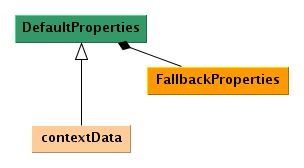
\includegraphics[height=3cm,width=6cm]{image/propertiescontext.png}
  		\caption{Fonctionnement du ContextData}
  		\label{propertiescontext}
\end{figure}



Context app
QUi est en fait le nom de l'application, le début du label des wikitty.
ça permet pendant l'évaluation d'allerchercher uniquement les wikitty par
nom qui sont directement sous le même label application mère.
ça permet d'éviter les collisions de nom entre wikitty 


\subsection{Ajout d'un mécanisme de login/logout}

Les couches sécurité des wikitty service s'occupe déjà d'un mécanisme de login
et d'une gestion des droits en fonction. Les utilisateurs sont stocker en tant
que wikitty dans la base et on peut attribué des droits à ces utilisateurs.
Ensuite via un wikitty service on peut se loger, sur une authentification on
récupére un jeton qui sera à passer pour chaque action, celà est géré par le
wikitty proxy qui encapsule le wikitty service.

Donc pour vérifier qu'une authentification s'est bien passé il faut regarder
dans le proxy si l'utilisateur est présent. Dans le cas de wikitty publication
au moment de l'action de login, délégué au proxy, on va stocker le jeton et
l'utilisateur dans la session.

Evidement le mécanisme de Logout lui nettoie simplement la session en la vidant
de ces informations.

Ensuite le fonction de la gestion de l'authentification se repose sur le
méchanisme d'intercepteur et de package de struts. On défini une pile
d'intercepteur personalisé qui en plus de la pile par defaut rajoute un
intercepteur d'authenfication qui vérifiera la présence des informations
utilisateur dans la session, et bloquera l'accès à la page demandé si
l'utilisateur n'est pas authentifié.

On définit que l'accès aux actions publication utilise cette pile d'intercepteur
qui gère l'authentification, c'est ainsi que fonctionne le méchanisme dans
wikitty publication.

\subsection{Amélioration des pages d'affichage et d'édition}

Les pages d'édition et d'affichage des wikitty étaient relativement simple, le
but étant une administration simple et efficace des wikitty. L'amélioration de
ces pages à consister en la correction des bugs présent déjà dans le prototype.

Par exemple le support pour les recherches dans wikitty dans la page view,
dans le prototype cette recherche était très limité et donc ne fonctionnait pas
très bien. De plus l'affichage des résultats nécessitait une amélioration.

Ensuite pour l'interface d'édition des wikitty j'ai intégré un décorateur de
Text Area qui permet une colorisation du contenu du champ, on peut choisir le
langage présent dans le champ pour avoir une colorisation, de l'indentation, des
outils de recherche/remplacer et d'autre, basiquement une sorte d'ide pour
faciliter le dévellopement de code dans les WikittyPubText.

% mettre screen shot du décorateur de textarea


\subsection{Mécanisme de multicontext}

Cette fonctionnalité consiste en fait à l'encapsulation par un wikitty service
de deux autres wikitty service, quelque soit leurs natures, c'est un 
WikittyFallbackService. On peut voir un schéma de fonctionnement sur la figure
\ref{diagmulticontext}

Ce multi contexte éxécute ses recherches un wikitty service principal, et
compléte ses recherches si besoin avec les données du wikitty service dit
fallback. A titre d'exemple si on effectue une recherche que l'on réclame un
résultat d'au moins 30 wikitty, si à l'issue de la recherche sur le wikitty 
service principal il n'y a pas 30 wikitty, alors on cherchera sur le service
fallback pour compléter la recherche. 

Ainsi si l'on cherche à retrouver un wikitty particulier avec son id, si il
se trouve sur le principal ça sera le wikitty du principal qui sera renvoyé, 
par contre si il ne se trouve pas sur celui si, on ira le chercher sur le second
service.

De même l'écriture s'effectue sur le service principale, on n'écrit pas sur le
service de fallback.

\begin{figure}[!ht]
  	%[height=12cm,width=15cm]
\centering
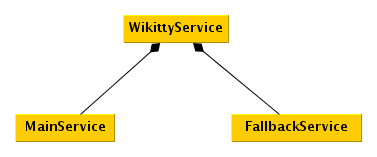
\includegraphics{image/multicontext.png}
  		\caption{Diagramme multicontexte}
  		\label{diagmulticontext}
\end{figure}


Son utilisation n'est pas nécessairement limité à Wikitty Publication, il s'agit
finalement d'une implémentation différente de l'interface wikitty service. 

Ce mécanisme peut permettre la surcharge d'un wikitty, dans le sens ou on peut
modifier un wikitty qui aura été chargé depuis le fallback, mais à la sauvegarde
il sera restaurer depuis le wikitty principal, puisque celui ci est prioritaire.

On peut avoir ainsi un wikitty service statique, et un autre dynamique, par
exemple le wikitty service statique qui serait partagé et utilisé par d'autre
wikitty service multicontext, une base commune de wikitty. 

Ce Wikitty Service à été pensé et écrit pendant l'enrichissement de la partie 
site de Wikitty Publication, l'idée d'utilisation d'un tel service, est la 
mutualisation d'une application dans un wikitty service, et que cette 
application utilise des données issue de d'autre service. On mutualise le code 
métier, de sorte que plusieurs clients puissent utiliser la même application, 
avec le même service, mais que leurs données soit sur leurs services, 
le service fallback contiendrait l'application et le service principal 
l'application.

\subsection{Intégration d'interface graphique}

Les applications éxécuté au sein de wikitty publication le seront à travers 
un navigateur web donc le résultat présenté dans un format compatible.
Donc générélament pour proposer des choix utilisateurs il faudra des interfaces
en html.

Le html peut être aisément intégré dans du javascript et quand l'évaluateur
evaluera le javacript et écrira le html contenu dans les variables javascript
mais cette solution rends l'écriture du code interface pénible.




%mettre un exemple de code ici.TODO

La solution la plus simple qui a été trouvé est d'avoir la possibilité d'écrire 
du html (pour le moment plus tard d'autre langage) et de faire comme si on était
dans une jsp, quand on a besoin d'écrire code on ouvre des balises : <\% \%>
ou <\%= \%> et on écrit le code correspondant.

Ce qui se passe derrière c'est que on inverse le code, ce qui se trouve entre
les balises devient du code exécutable, et ce qui se trouve autour se retrouve
décoré. Tout simplement comme si initialement le html avait été intégré dans
le code d'un langage interprété par publication.

Une autre solution était envisagé, qui voulait considérer le html comme un langage
supporté par publication, et extraire les éléments de binding mais c'était plus 
compliqué.

Utilisation des mimes types composé pour déterminer un prétraitement

